\documentclass[12pt,a4paper]{article}
\usepackage{times}
\usepackage{durhampaper}
\usepackage{harvard}
\usepackage{graphicx}
\usepackage{float}
\usepackage{flafter}
\usepackage{nameref}
\usepackage[htt]{hyphenat}

\citationmode{abbr}
\bibliographystyle{agsm}

\let\OLDthebibliography\thebibliography
\renewcommand\thebibliography[1]{
  \OLDthebibliography{#1}
  \setlength{\parskip}{0pt}
  \setlength{\itemsep}{0pt plus 0.3ex}
}

\title{Defeating MAC address randomisation: A hybrid, multi-layer approach for indoor location-based services}
\author{}
\student{Maximilian Grimmett}
\supervisor{Dr Eleni Akrida}
\degree{MEng Computer Science}

\newcommand{\absdiv}[1]{%
  \par\textbf{#1}\quad\ignorespaces \\
}

\date{}

\begin{document}

    \maketitle

    \begin{abstract}
        \absdiv{Context/Background}
        Recently, location-based indoor positioning services using 802.11 (Wi-Fi) have seen a rise in popularity of MAC randomisation to prevent tracking of individual devices throughout their stay.

        \absdiv{Aims}
        Primarily, this paper looks to implement a system that combines previous techniques for MAC \\ de-randomisation at different layers of the OSI model and conduct comparative research evaluating it relative to their individual use.
        Secondly, this paper looks to generalise these techniques to consider and evaluate groups of devices moving between different 802.11 nodes of the same network.
        Additionally, to enable such comparisons, this paper aims to produce a novel, modular testing and evaluation framework which uses Monte Carlo simulation to generate realistic, real-time data.
        
        \absdiv{Method}
        Due to the ethical implications of collecting potentially identifiable real-world data and the impracticality of doing so in a controlled environment, a real-world study is not suitable.
        While applicable real-world datasets do exist, they do not encompass all the fields required at the different levels of abstraction used by the proposed hybrid system.
        Instead, this paper proposes the use of Monte Carlo simulation of devices with and without MAC randomisation.

    \end{abstract}

    \begin{keywords}
        Location-based services, MAC randomisation, dynamic networks, privacy-preservation.
    \end{keywords}
    % \pagebreak

    \section{Introduction}\label{sec:introduction}
    % Between 2 and 3 pages
% General project background, research question, and objectives.
% About 5-10 references

\subsection{Background and Motivation}\label{sec:motivation-and-background}

\subsubsection{Location-based Services}\label{sec:location-based-services}

Location-based Services (LBSs) is a large field which has seen an explosion in academic and industry interest~\cite{Junglas2008} since the beginning of the 21st century.
Broadly speaking, it covers information-technology services involved in the collection, analysis and application of any data that tracks the location of either objects, devices or people.
Much of the interest has stemmed from its potential for interdisciplinary use and insight into geographical social trends and tendencies.
It has seen applications in security, health and marketing (mainly for advertising).

Historically, positioning in LBSs has been restricted to use by those who own the infrastructure, namely telecom operators.
~\citeasnoun{Bellavista2008} note the past monopolistic infrastructure-centric nature of both indoor and outdoor localisation and describe this as the shift from operator-centric to user-centric management of LBSs.

As they cover such a wide range of services, LBSs can be grouped by certain characteristics and scopes of usage.
Within the field of localisation, an important divide is made between indoor and outdoor LBSs.
Outdoor LBSs primarily make use of GPS and telecom towers for positioning.
A large example of an outdoor LBS which uses GPS is satellite navigation and social media geotagging which, as of 2013 saw a large usage uptake~\cite{zickuhr2013}.

On the other hand, GPS and telecom tower triangulation is not suitable for indoor positioning.
Even though its possible to receive GPS signal indoors with modern hardware, studies such as \cite{merry2019smartphone} have shown it to be accurate to between 7 and 13 metres outdoors.
This kind of accuracy is only enough to place a device in a building or potentially a large room.
Additionally, GPS elevation is only accurate to between 10 and 20 metres, which is not enough to accurately detect what floor a device is on.
Hence, for better lateral/longitudinal and vertical accuracy, a different localisation technique is required for indoor LBSs.

\subsubsection{Indoor Position Tracking}\label{sec:indoor-position-tracking}

Indoor positioning, or indoor localisation, typically involves tracking the location of people, or groups of people as they move around some premises.
The hardware and software used to achieve this is called an indoor positioning system (IPS), sometimes also referred to as an indoor localisation system (ILS).

IPSs come in many forms and can be broadly split into two groups: computer vision (CV)-based and device-based.
CV-based IPSs have seen increased use recently in line with advancements in state-of-the-art CV object-tracking and facial-recognition methods.
Device-based IPSs typically use wireless technologies such as 802.11 (Wi-Fi)~\cite{ieee1997}, Bluetooth, Bluetooth Low Energy (BLE) and RFID~\cite{S.Shen2020}.
Despite being an exciting technology, a large problem with CV-based IPSs is that they present a much greater privacy risk than device-based IPSs.
This is not only due to the potential for (and incentivised use of) facial recognition, but also the ethical issues with regards to the recording (and storing of recordings) of individuals.

An advantage of 802.11 IPSs is that tracking can be done completely passively.
Almost all modern smartphones have Wi-Fi capability and are constantly sending probe requests to scan for Access Points (APs).
Because of this, their implementation and use of the protocol is all that is required to detect devices.

Received Signal Strength (RSS) is a measure, in decibels, of how strong a signal between two devices are -- these devices are typically a smartphone and a wireless 802.11 AP.
Since RSS is inversely proportional to distance, obtaining the RSS from three APs is enough to triangulate a mobile device to a reasonable degree of accuracy, this is demonstrated in Figure~\ref{fig:triangulation}.
Some IPSs additionally make use of Received Response Time (RRT) and some APs contain additional hardware to calculate Angle of Arrival (AOA), both of which can be used to further increase localisation accuracy.

\begin{figure}[!ht]
    \centering
    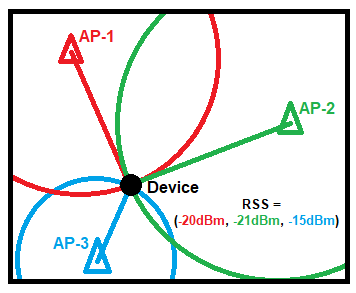
\includegraphics[scale=0.4]{figures/triangulation.png}
    \caption{Triangulation of a mobile device from three APs using RSS.}
    \label{fig:triangulation}
\end{figure}

\subsubsection{MAC Address Randomisation}\label{sec:mac-randomisation}

The operating system of a device is ultimately responsible for implementing the protocols it uses.
As such, there is no way to enforce a device sending its true physical Media Access Control (MAC) address.
This enables the operating system to handle 802.11 communication (including sending probe requests and connecting) with a MAC address of their choice.

Consider the two most widely used operating systems for mobile smartphones: iOS and Android.
Both iOS 8, released in 2014, and Android 6, released in 2015, introduced MAC randomisation in probe requests as the default behaviour.
Since then, both iOS 14, released in 2020, and Android 9, released in 2018, implement full MAC randomisation when connecting to networks.
Whereas the iOS implementation rotates the randomised MAC address every 24 hours, Android retains the same (originally randomised) address per 802.11 SSID\@.
In 2019, Android 10 set this as the default behaviour (as does iOS 14).

While these measures have little practical impact on the user experience when using guest Wi-Fi provided by businesses, it is catastrophic for LBSs which rely on 802.11 probe requests to identify users and their location.
In practice, this means that LBSs are, at best, able to pinpoint the location of a device but not detect its movement over a time period (where MAC randomisation for probe requests is on a fixed timer).
At worst, they are not able to pinpoint a device at all (when MAC addresses are randomised between probe requests).

\subsection{802.11 fingerprinting}\label{sec:wifi-fingerprinting}

Since before the widespread adoption of MAC randomisation, passive 802.11 fingerprinting has been a hot topic for research~\cite{Pang2007}.
In the context of the 802.11 protocol, fingerprinting may either refer to the spatio-temporal identification of individual devices or the pre-processing of specific buildings to calibrate or improve localization success rate of an algorithm.
For the remainder of this paper, assume fingerprinting refers to the former unless otherwise stated.
Additionally, take `MAC de-randomisation' to mean the process of uniquely identifying a device across space and time.

This paper considers two primary forms of fingerprinting techniques for MAC de-randomisation: implicit identifier fingerprinting proposed by~\citeasnoun{Pang2007} and timing attacks proposed by~\citeasnoun{Matte2016} (both of which work on the physical-layer of the OSI model).
A third technique that is considered, which does not involve fingerprinting, works on the link-layer of the OSI model and will be referred to as MAC vendor analysis.
Broadly-speaking, implicit identifier fingerprinting exploits minor differences in manufacturing within the tolerances of mobile devices to uniquely identify them.
Timing attacks use the Inter-frame Arrival Times (IAT) of sets of frames to group them by likelihood of them being sent from the same device.
MAC vendor analysis uses knowledge of how manufacturers assign the lower-order bytes of addresses to devices to infer information about the device.
These are discussed in greater detail as part of Sections~\ref{sec:related-work} and~\ref{sec:solution}.

\subsection{Aims}\label{sec:aims}

The primary objective of this paper is to compare a hybrid implementation consisting of implicit-identifier 802.11 fingerprinting, timing attacks and vendor analysis compared to their individual use.
To assist with this, the paper also aims to produce a Monte Carlo-based location data simulation method to benchmark and test the systems.
Finally, this paper aims to evaluate the hybrid tracking technique when generalised to groups of moving devices.

This research aims to address the following questions:
\begin{enumerate}
    \itemsep-0.5em
    \item What are the differences and similarities between the performance of 802.11 fingerprinting, timing attacks and MAC vendor analysis applied independently compared to them combined into one hybrid method?
    \item How well does this hybrid method generalise to groups of individuals?
    \item How well do these different methods work when applied across the different versions of 802.11?
    \item How can real-world location data be simulated for a controlled testing and evaluation environment?
\end{enumerate}

    % \pagebreak

    \section{Related Work}\label{sec:related-work}
    % About 2 pages

This section presents a survey of existing work on the problems that this project addresses.  it should be between 2 to 4 pages in length.  The rest of this section shows the formats of subsections as well as some general formatting information for tables, figures, references and equations.

\subsection{Main Text}
The font used for the main text should be Times New Roman (Times) and the font size should be 12.  The first line of all paragraphs should be indented by 0.25in, except for the first paragraph of each section, subsection, subsubsection etc. (the paragraph immediately after the header) where no indentation is needed.

\subsection{Figures and Tables}
In general, figures and tables should not appear before they are cited.  Place figure captions below the figures; place table titles above the tables.  If your figure has two parts, for example, include the labels ``(a)'' and ``(b)'' as part of the artwork.  Please verify that figures and tables you mention in the text actually exist.  make sure that all tables and figures are numbered as shown in Table \ref{units} and Figure 1.
% sort out your own preferred means of inserting figures

\begin{table}[htb]
    \centering
    \caption{UNITS FOR MAGNETIC PROPERTIES}
    \vspace*{6pt}
    \label{units}
    \begin{tabular}{ccc}\hline\hline
        Symbol & Quantity & Conversion from Gaussian \\ \hline
    \end{tabular}
\end{table}

\subsection{References}
The list of cited references should appear at the end of the report, ordered alphabetically by the surnames of the first authors.  References cited in the main text should use Harvard (author, date) format.  When citing a section in a book, please give the relevant page numbers, as in \cite[p293]{budgen}.  When citing, where there are either one or two authors, use the names, but if there are more than two, give the first one and use ``et al.'' as in  , except where this would be ambiguous, in which case use all author names.

You need to give all authors' names in each reference.  Do not use ``et al.'' unless there are more than five authors.  Papers that have not been published should be cited as ``unpublished'' \cite{euther}.  Papers that have been submitted or accepted for publication should be cited as ``submitted for publication'' as in \cite{futher} .  You can also cite using just the year when the author's name appears in the text, as in ``but according to Futher \citeyear{futher}, we \dots''.  Where an authors has more than one publication in a year, add `a', `b' etc. after the year.

    % \pagebreak

    \section{Solution}\label{sec:solution}
    % About 2.5 pages
% Up to 2 references

The core methodology this paper will implement is a purely quantitative mix between comparative and evaluative research, with the generation of data being slightly exploratory.

\subsection{Testing and Evaluation Framework}\label{sec:testing-framework}

This section will present the proposed Monte Carlo-based data generation, describe the implementation of the testing and evaluation framework and discuss the measures of effectiveness used for comparison.

\subsubsection{Data Generation with Monte Carlo Simulation and Randomised Algoritms}

Due to the previously discussed ethical and privacy issues with real-world data collection and impracticality of setting up a real-world 802.11 study, a seemingly simple solution is to instead generate the data through Monte Carlo simulation.
Additionally, while there are plenty of existing datasets, they do not contain all the fields required for the application of each of the independent methods.
Because of this, the implementation of a Monte Carlo simulation to generate location data representative of devices with, and without, MAC randomisation would not only be useful for this study, but also future research (potentially in related fields).
This is combined into a testing and evaluation framework that enables the modular insertion or removal of the methods shown in Figure 3 (plus the hybrid model with all of them combined).

Pinpointing location with 802.11 is a more complex technical issue than the implementation of triangulation alone.
Much like with GPS, the indoor environment presents localisation difficulty due to walls and other obstructions.
A typical existing wireless infrastructure may consist of one access point per floor, or, at best, one per room.
If such a system was transformed to include an IPS without additional hardware modification, it would result in high inaccuracy when estimating the location of a device.
Because of this, the Monte Carlo simulation will emulate an ideal testing environment, where there are multiple access points in a single room.

The Monte Carlo method is a class of algorithms which leverage random sampling to obtain numerical results~\cite{raychaudhuri2008}.
They are well-suited to simulating physical models due to their near-nondeterministic nature.
This makes them ideal for simulating physical-layer characteristics such as those used by implicit identifier fingerprinting.
Additionally, they can be used to simulate the frame emission times required by the timing attack.

 simulations is the employment of random-based algorithms to generate both true and randomised MAC addresses.
These can then be used by the timing attack as part of its fingerprinting and be sent for MAC vendor analysis.

Finally, each simulation (whether considering one or more devices) is run a fixed number of times.
The exact number of times they are run is determined experimentally trough trial and error until the results converge to within a pre-determined error margin.

\subsubsection{Software Framework}

Each de-randomisation technique is independently implemented as a module extending a \texttt{DerandomisationTechnique} abstract base class, specifying the location data fields they require as input from the framework.
At runtime, through dependency injection, the framework provides the requested data (and continues to update it as the simulation runs).
It then calls to an interface method implemented by the technique to return the MAC addresses.

To guarantee more valid, truthful location-data output from the Monte Carlo simulation, its hyperparameters and probability distributions are fine-tuned by running the independent techniques and tweaking them to closely match the results obtained in their respective papers.

The implementation provided by the framework of the 802.11 protocol is designed to enable modularity.
For the reasons mentioned earlier, this enables testing of how well the various techniques work on different versions of the 802.11 protocol.
An object-oriented approach is proposed whereby an abstract base class, \texttt{Simulated80211}, is inherited by concrete classes which implement the respective version of 802.11 (for example, \texttt{Simulated80211b} for the 1999 version, or \texttt{Simulated80211ax} for the 2021 version).
It is within these concrete classes that the Monte Carlo simulation and randomised algorithms are implemented.
This is then further abstracted to have \texttt{Simulated80211} extend the abstract base class \texttt{WirelessProtocol}, allowing any protocol to be used.
Because of this, the concrete implementation of the protocol corresponding to the one being tested (or used for evaluation) is instantiated at runtime, and can be freely swapped out as required (even for a real-world source).

With this in mind (and using the separation of concerns principle), the concepts of premises (\texttt{Premises}), devices (\texttt{Device}), APs (\texttt{AccessPoint}) and IPS software (\texttt{IpsSoftware}) are defined as different entities.
In the 3D model, for simplicity, premises are represented by a rectangular cuboid of arbitrary size, and both APs and devices are represented by a single point within the bounds of the premises.
Implementation-wise, a \texttt{Premises} only stores its bounding-box, a \texttt{Device} and \texttt{AccessPoint} both store a three-dimensional position vector and a \texttt{WirelessProtocol} and \texttt{IpsSoftware} stores a \texttt{DerandomisationTechnique} instance.
All of these are externally managed by a \texttt{SimulationManager}.
The manager maintains a list of \texttt{EvaluationMetric} instances which use the results to calculate the metrics listed below.
Because the manager has access to both the simulated results and true location assignments, it sends them into each \texttt{EvaluationMetric} and outputs the results.

\subsubsection{Measure of Effectiveness}

The primary measure of how effective each method is will be based upon the percentage of devices successfully tracked over discrete time frames.
The reason for using this is because it closely matches the real-world application of tracking users’ locations across space and time.
In addition to their use in simulation calibration, the other metrics from the original papers can be used for the hybrid system and compared as a supplement to the primary spatio-temporal measure of success.
Finally, as the framework is a controlled environment, the simulation manager is able to undertake performance profiling for speed and memory usage on the simulated techniques.
This performance information is also useful knowledge for real-world application because it can be used to determine required hardware specifications.

\subsection{Hybrid System}\label{sec:hybrid-system}

This section will go into more detail on how the three MAC de-randomisation techniques fit together to form the hybrid system and how it fits with the software framework.

\subsubsection{Overview}

Figure~\ref{fig:solutionstack} shows a high-level diagram-description demonstrating the modularity and the layers at which each technique resides in the OSI model.
Each layer is directly related to the data it requires: implicit identifier fingerprinting requires low-level parameters such as packet size, (encrypted) packet data and 802.11 options, timing attacks require low-level parameters such as probe request data and IAT, and higher-level parameters like MAC address, and this implementation of MAC vendor analysis requires only the broadcast MAC address.

\begin{figure}[!ht]
    \centering
    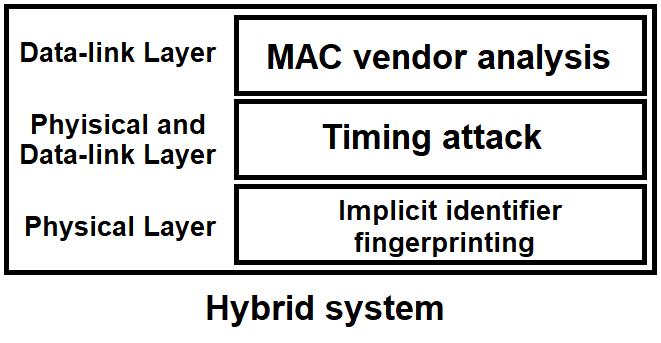
\includegraphics[scale=0.25]{figures/solutionstack.png}
    \caption{Illustration of the proposed hybrid system, and the OSI layers it encompasses.}
    \label{fig:solutionstack}
\end{figure}

\subsubsection{Software Implementation}

The modular approach described in~\nameref{sec:testing-framework} continues to apply to the hybrid system.
The concrete class \texttt{HybridTechnique} extends \texttt{DerandomisationTechnique} and contains one field for each independent technique.
As it extends the \texttt{DerandomisationTechnique} base class, it can be substituted in at runtime as if it were its own technique.
All it has to do is implement a way to pass required arguments and the simulated location-data down to the respective techniques.

    % \pagebreak

    \section{Validity}\label{sec:validity}
    % Maximum 1 page
    % \pagebreak

    \section{Results}\label{sec:results}
    % Intentionally left blank


    \section{Evaluation}\label{sec:evaluation}
    % Intentionally left blank


    \section{Conclusion}\label{sec:conculsion}
    % Intentionally left blank


    % \nocite{*}

    {\footnotesize
    \bibliography{projectpaper}}

\end{document}